\documentclass[ignorenonframetext,]{beamer}
\setbeamertemplate{caption}[numbered]
\setbeamertemplate{caption label separator}{: }
\setbeamercolor{caption name}{fg=normal text.fg}
\beamertemplatenavigationsymbolsempty
\usepackage{lmodern}
\usepackage{amssymb,amsmath}
\usepackage{ifxetex,ifluatex}
\usepackage{fixltx2e} % provides \textsubscript
\ifnum 0\ifxetex 1\fi\ifluatex 1\fi=0 % if pdftex
\usepackage[T1]{fontenc}
\usepackage[utf8]{inputenc}
\else % if luatex or xelatex
\ifxetex
\usepackage{mathspec}
\else
\usepackage{fontspec}
\fi
\defaultfontfeatures{Ligatures=TeX,Scale=MatchLowercase}
\fi
\usetheme{Singapore}
% use upquote if available, for straight quotes in verbatim environments
\IfFileExists{upquote.sty}{\usepackage{upquote}}{}
% use microtype if available
\IfFileExists{microtype.sty}{%
\usepackage{microtype}
\UseMicrotypeSet[protrusion]{basicmath} % disable protrusion for tt fonts
}{}
\newif\ifbibliography

% Prevent slide breaks in the middle of a paragraph:
\widowpenalties 1 10000
\raggedbottom

\AtBeginPart{
\let\insertpartnumber\relax
\let\partname\relax
\frame{\partpage}
}
\AtBeginSection{
\ifbibliography
\else
\let\insertsectionnumber\relax
\let\sectionname\relax
\frame{\sectionpage}
\fi
}
\AtBeginSubsection{
\let\insertsubsectionnumber\relax
\let\subsectionname\relax
\frame{\subsectionpage}
}

\setlength{\parindent}{0pt}
\setlength{\parskip}{6pt plus 2pt minus 1pt}
\setlength{\emergencystretch}{3em}  % prevent overfull lines
\providecommand{\tightlist}{%
\setlength{\itemsep}{0pt}\setlength{\parskip}{0pt}}
\setcounter{secnumdepth}{0}

\title{California Scorpionfish 2017 Assessment}
\subtitle{Biology and Data}
\author{Melissa H Monk\(^1\), \and Xi He\(^1\), \and John Budrick\(^2\)}
\institute{\(^1\)Southwest Fisheries Science Center \and \(^2\)California Department of Fish and Wildlife}
\date{STAR Panel July 24-28, 2017}

\begin{document}
\frame{\titlepage}

\begin{frame}
\tableofcontents[hideallsubsections]
\end{frame}

\begin{frame}

\end{frame}

\section{Tables}\label{tables}

\FloatBarrier
\newpage

\FloatBarrier

\FloatBarrier

\FloatBarrier

\FloatBarrier

\FloatBarrier

\FloatBarrier

\FloatBarrier

\FloatBarrier

\FloatBarrier

\begin{landscape}

\end{landscape}

\FloatBarrier

\newpage

\FloatBarrier

\FloatBarrier

\newpage

\begin{landscape}

\end{landscape}

\newpage

\begin{landscape}

\end{landscape}

\newpage

\begin{landscape}

\end{landscape}

\FloatBarrier

\newpage

\newpage

\FloatBarrier

\section{Background}\label{background}

\begin{frame}{California scorpionfish \emph{Scorpaena guttata}}

\begin{itemize}
\tightlist
\item
  Distributed from central California to Punta Eugenia, Baja Mexico
\item
  Rarely observed north of Pt. Conception
\item
  Observed from the intertidal to 600 ft, preferred depth range from
  20-450 ft
\item
  Demersal, found over both hard and soft bottom
\item
  Exhibit aggregating behavior (spawning and non-spawning)
\end{itemize}

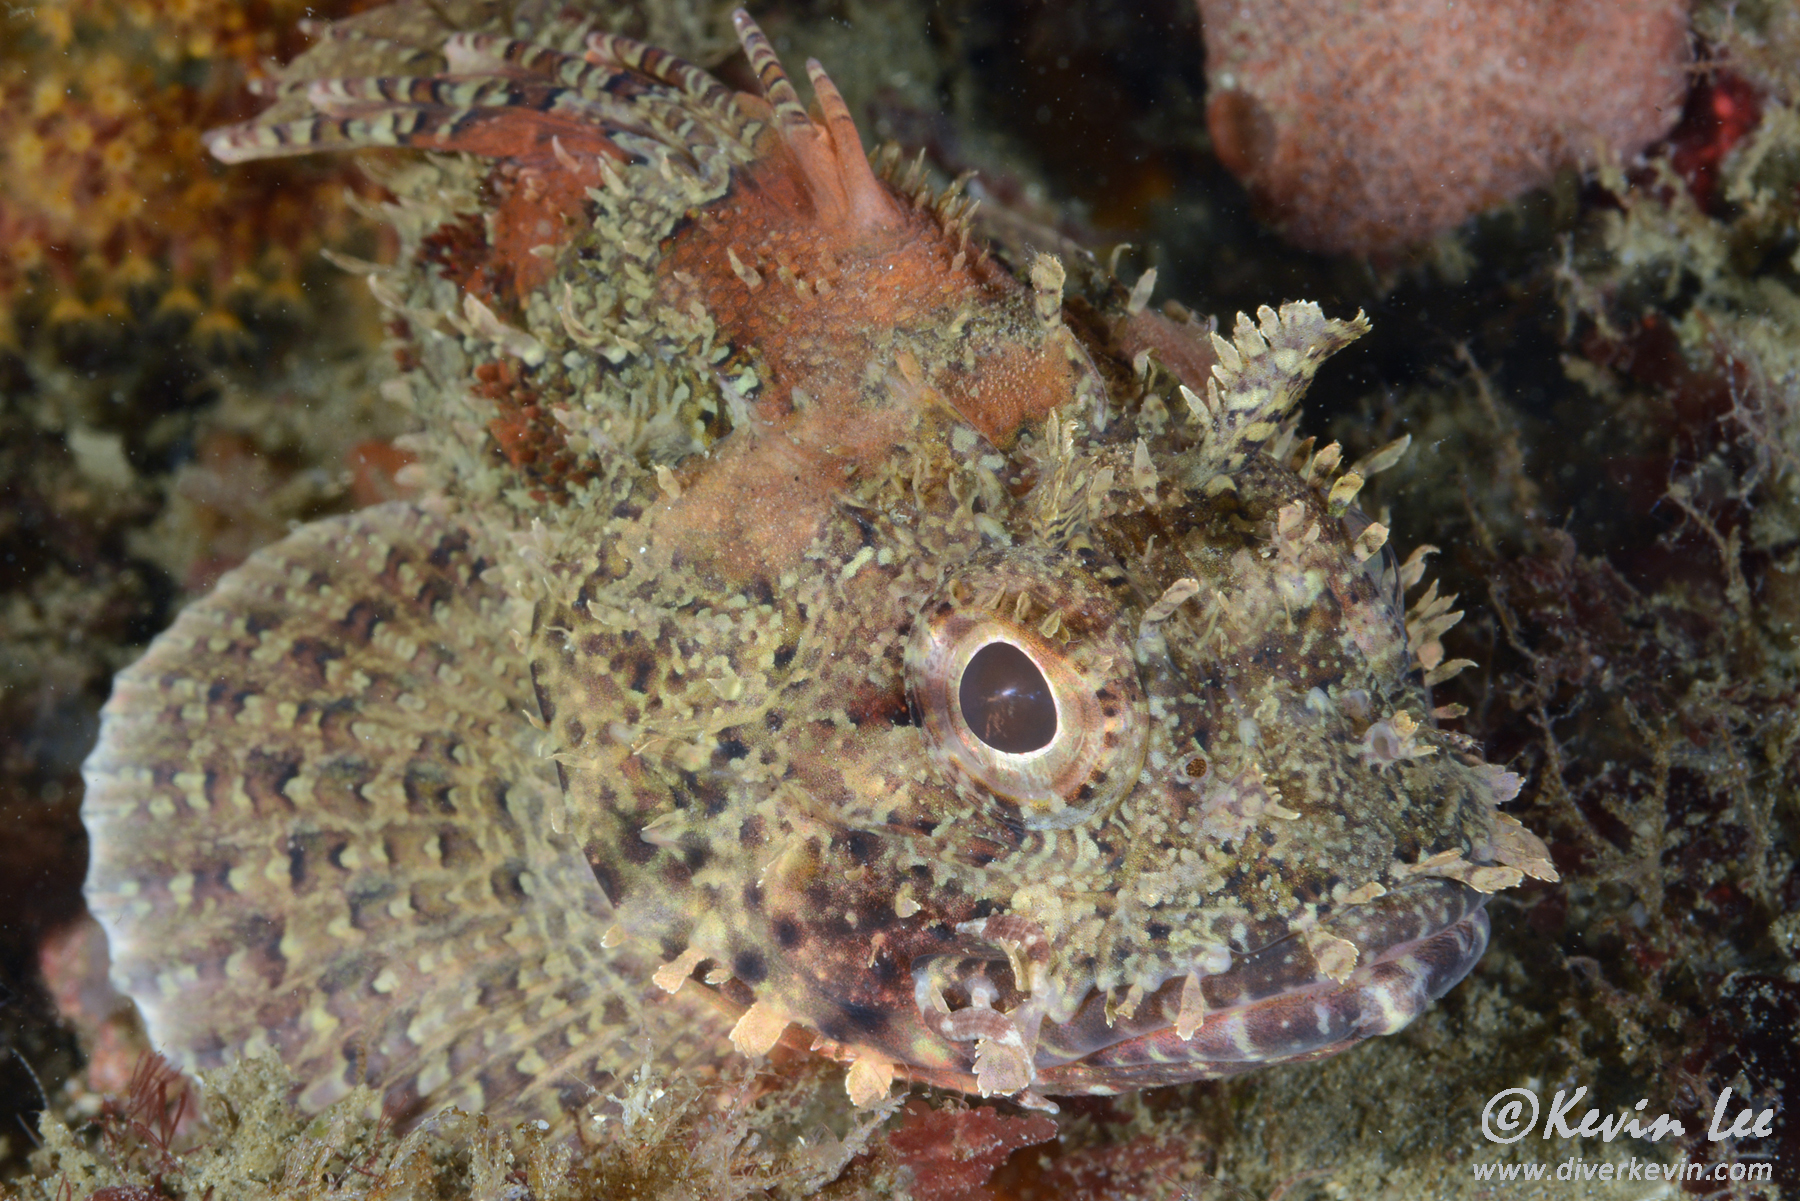
\includegraphics[width=.5\textwidth, right]{cover_photo}

\end{frame}

\section{Biology}\label{biology}

\begin{frame}{Length-at-age}

\end{frame}

\begin{frame}{Maturity}

\end{frame}

\begin{frame}{Weight-at-length}

\end{frame}

\begin{frame}{Natural mortality}

\end{frame}

\begin{frame}{Steepness}

\end{frame}

\begin{frame}{Summary of Data used in the 2017 Assessment}

\end{frame}

\section{Removals}\label{removals}

\begin{frame}{Total Removals}

\end{frame}

\begin{frame}{Commercial Landings by Fleet}

\end{frame}

\begin{frame}{Recreational Landings by Fleet}

\end{frame}

\section{Index Data}\label{index-data}

\begin{frame}{Summary of Indices}

\begin{itemize}
\tightlist
\item
  All of the methods used to standardize indices have been endorsed by
  the SSC
\end{itemize}

\begin{table}[ht]
\centering
\scalebox{0.7}{
\begin{tabular}{p{2.5in}p{0.8in}p{.4in}p{2in}}
  \hline
Name & Years & Fishery ind. & Method \\ 
  \hline
Recreational PR dockside CPUE & 2004-2016 & No & delta-GLM (bin-lognormal) \\ 
  CPFV logbook CPUE & 1980-2016 & No & negative binomial \\ 
  Onboard observer discard catch CPUE & 2002-2016 & No & delta-GLM (bin-lognormal) \\ 
  Sanitation district CPUE & 1970-2016 & Yes & delta-GLM (bin-lognormal) \\ 
  NWFSC trawl survey CPUE & 2003-2016 & Yes & VAST \\ 
  CSUN/VRG Gillnet survey CPUE & 1995-2008 & Yes & delta-GLM (bin-lognormal) \\ 
  Southern Califrnia Bight trawl survey CPUE & '94, '98, '03, '08, '13 & Yes & delta-GLM (bin-lognormal) \\ 
  Onboard observer retained catch CPUE & 2002-2016 & No & delta-GLM (bin-lognormal) \\ 
   \hline
\end{tabular}
}
\end{table}

\end{frame}

\begin{frame}{Recreational Private Boat Index}

\end{frame}

\begin{frame}{Recreational Party/Charter Boat Index (Logbook)}

\end{frame}

\begin{frame}{Recreational Dead Discard Index}

\end{frame}

\begin{frame}{Recreational Party/Charter Retained Catch Index}

\end{frame}

\begin{frame}{Sanitation Districts Survey Index}

\begin{table}[ht]
\centering
\scalebox{0.9}{
\begin{tabular}{lrrrrr}
  \hline
Program & 0-24 m & 25-49 m & 50-74m & 100+ m & Total \\ 
  \hline
City of Los Angeles & 120 &   0 & 1372 &   0 & 1492 \\ 
  Los Angeles County & 687 &   0 & 5879 & 450 & 7016 \\ 
  Orange County & 161 & 669 & 2157 &  48 & 3035 \\ 
  City of San Diego &   0 & 404 & 333 & 829 & 1566 \\ 
   \hline
\end{tabular}
}
\end{table}

\end{frame}

\begin{frame}{Sanitation Districts Survey Index}

\end{frame}

\begin{frame}{Sanitation Districts Survey Index}

\end{frame}

\begin{frame}{NWFSC Trawl Survey Index}

\end{frame}

\begin{frame}{Gillnet Survey Index}

\end{frame}

\begin{frame}{Southern California Bight Trawl Survey Index}

\end{frame}

\section{Composition Data}\label{composition-data}

\end{document}
